\chapter{Dataset e Setup Sperimentale}
    \section{Obiettivi della fase iniziale}
        Questa prima fase del progetto ha conseguito i seguenti obiettivi:
            \begin{enumerate}
                \item Costruire un test set realistico, bilanciato e rappresentativo per la valutazione delle performance facciali.
                \item Valutare le prestazioni del modello NN1 in condizioni non perturbate, per stabilire una baseline di riferimento.
                \item Definire un ambiente stabile e riproducibile per l’esecuzione controllata di attacchi adversarial e successive difese.
            \end{enumerate}

        \noindent I risultati ottenuti in questa fase costituiscono la base sperimentale su cui si innesteranno, nei capitoli successivi, l’analisi degli attacchi e l’efficacia delle contromisure proposte.

    \section{Ambiente di sviluppo}
        Tutte le sperimentazioni sono state condotte in ambiente separato \textit{conda} (\texttt{anaconda} o \texttt{miniconda}) utilizzando \texttt{Python 3.10}, sfruttando \textit{Jupyter Notebook}, \texttt{PyTorch} come framework di deep learning e \texttt{Adversarial Robustness Toolbox (ART)} per la generazione e gestione degli attacchi adversarial. I notebook sono stati sviluppati ed eseguiti su \textit{Visual Studio Code}, sfruttando una GPU.
        Di seguito si elencano le principali dipendenze utilizzate:
            \begin{itemize}
                \item \texttt{torch==2.x}, \texttt{torchvision}
                
                \item \texttt{numpy}, \texttt{matplotlib}
                
                \item \texttt{adversarial-robustness-toolbox}
                
                \item \texttt{facenet-pytorch}, \texttt{tensorflow}
            \end{itemize}

    \section{VGG-Face2 e costruzione del test set}
        Per valutare la robustezza del sistema di riconoscimento facciale, è stato utilizzato un modello (\texttt{InceptionResnetv1}) pre-addestrato sul dataset \texttt{VGG-Face2}, uno dei benchmark più noti in ambito face recognition. Questo dataset contiene oltre 3 milioni di immagini raccolte dal web e suddivise in più di 9.000 identità, con una forte variabilità in termini di età, etnia, pose e condizioni di illuminazione.
        Ai fini di questo progetto, come da requisiti, sono state selezionate manualmente \textbf{100 identità} dal training set del dataset, ciascuna rappresentata da almeno \textbf{20 immagini}, per un totale complessivo di \textbf{2408 immagini}.
        Per garantire variabilità intra-classe (espressioni, pose, sfondi) e inter-classe (etnie, sesso, età), le immagini sono state accuratamente filtrate. Durante una fase preliminare di cleaning sono stati rimossi file duplicati, volti oscurati o mal ritagliati.
        Tale test set è stato utilizzato sia per la valutazione iniziale delle performance, sia come base per generare gli \textit{adversarial samples}.
        Il test set è stato organizzato secondo la struttura prevista da \texttt{torchvision.datasets.ImageFolder}, con una directory principale e una sottocartella per ciascuna identità (es. \texttt{dataset/Test\_set/n000202/}, \texttt{dataset/Test\_set/n000201/}, \ldots), rendendo agevole il caricamento e l’etichettatura automatica.
            \begin{figure}[H]
                \centering
                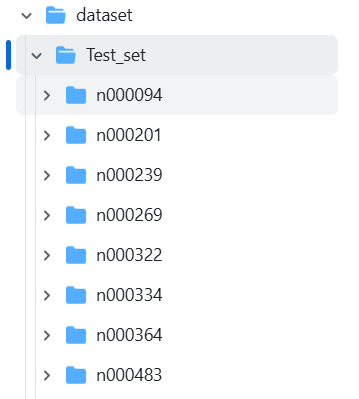
\includegraphics[width=0.55\textwidth]{images/Test_set.png}
                \caption{Test set organization}
            \end{figure}

        \noindent Durante la fase di importazione con \texttt{PyTorch}, per rendere le immagini conformi ai vincoli del modello riguardo gli input, sono state applicate una serie di trasformazioni:
            \begin{itemize}
                \item Resize a $160 \times 160$ pixel, come richiesto dal modello \texttt{InceptionResnetV1}, che accetta in input immagini quadrate di tale dimensione poichè risulta essere ottimizzato per questa risoluzione;
                \item Conversione in tensori;
                \item Normalizzazione con \texttt{mean} e \texttt{std} impostati a $[0.5, 0.5, 0.5]$
            \end{itemize}
            
        \noindent Il caricamento è stato gestito tramite un \texttt{DataLoader} con \texttt{batch\_size = 32} e \texttt{shuffle = False}, al fine di mantenere fisso l’ordine delle immagini per il confronto tra predizioni clean e adversarial. \\            
        
        \noindent \textbf{Distribuzione del test set:}
            \begin{itemize}
                \item Numero totale identità: 100
                \item Numero medio di immagini per identità: 24.08
                \item Dimensione media immagine: $160 \times 160 \times 3$
            \end{itemize}

    \section{Modello NN1}
        Il modello di partenza (denominato \textbf{NN1}) è una rete neurale convoluzionale profonda, basata sull’architettura \texttt{InceptionResnetV1}. Questo modello è stato pre-addestrato sul dataset \texttt{VGG-Face2} ed è reso disponibile tramite la libreria \texttt{facenet-pytorch}. È progettato per il riconoscimento facciale e restituisce, per ogni immagine in input, un vettore di \textbf{512 caratteristiche} (embedding) che rappresentano la firma numerica del volto nel dominio euclideo.
        A differenza dell’uso canonico in FaceNet (dove si confrontano direttamente gli embedding tra volti), in questo progetto il modello è stato utilizzato in modalità \verb|classify=True|, che abilita un layer di classificazione finale su 8.631 identità del dataset \texttt{VGG-Face2}. Le etichette corrispondenti ai samples presenti nel dataset sono state ottenuto caricando il file di riferimento \texttt{rcmalli\_vggface\_labels\_v2.npy}, reso disponibile dall'omonima repository Github. Infine, il modello così ottenuto è stato spostato, se disponibile, sulla GPU, per ridurre i tempi di calcolo.
        A partire dalla struttura del test set, le immagini sono state caricate e preprocessate tramite le trasformazioni descritte in precedenza. Ogni immagine è stata associata alla rispettiva etichetta di classe, secondo l’organizzazione delle sottocartelle prevista da ImageFolder. Per ottimizzare i tempi di esecuzione nelle iterazioni successive, i tensori contenenti immagini (\texttt{x\_test}) e label (\texttt{y\_test}) sono stati salvati in un file \texttt{.pt}, evitando così la necessità di ricostruire il dataset a ogni avvio.
        Durante la valutazione, il modello è stato utilizzato in modalità \texttt{eval()}, senza aggiornamento dei pesi, al fine di valutarne la robustezza così com'è, senza alcun fine-tuning. La fase di testing della rete originale ha previsto l’iterazione sull’intero test set, durante la quale ciascuna immagine è stata elaborata dal modello per produrre una predizione. Per ogni immagine, è stata selezionata la classe corrispondente alla probabilità massima in output, mentre la classe reale è stata recuperata dal test set di riferimento. La predizione è stata poi confrontata con la label reale per verificarne la correttezza.
        L’intero processo è stato eseguito all’interno di un blocco \texttt{torch.no\_grad()}, che disattiva il calcolo del gradiente durante l’inferenza, riducendo il consumo di memoria e velocizzando l’esecuzione. Al termine, l’accuratezza è stata calcolata come rapporto tra il numero di predizioni corrette e il numero totale di immagini nel test set, restituendo così il valore percentuale finale di accuratezza del classificatore.
        Nello specifico, l’accuratezza ottenuta sul test set “clean” (non perturbato) è stata pari al \textbf{92{,}32\%}, con \textbf{2.223} predizioni corrette su un totale di \textbf{2.408} immagini.
        Questa configurazione ha permesso di utilizzare NN1 come solido punto di riferimento per confrontare l’impatto degli attacchi avversari nei capitoli successivi.